% 2005 年上海卷文科普通卷第 21 题：抛物线、焦点及垂线关系示意（不按比例）。
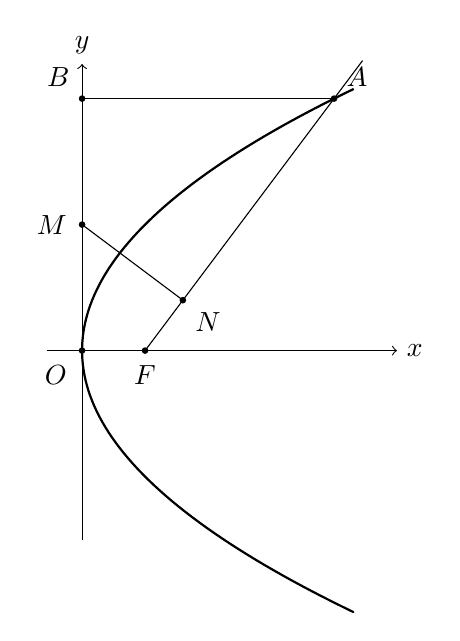
\begin{tikzpicture}[x=0.8cm,y=0.8cm,line cap=round,line join=round]
  % 以 y^2=4x 仅作形状示意；题面未给出 p 的数值。
  \draw[->] (-0.55,0)--(5.0,0) node[right] {$x$};
  \draw[->] (0,-3.0)--(0,4.55) node[above] {$y$};
  \draw[thick,domain=-4.15:4.15,samples=100] plot ({\x*\x/4},{\x});

  % A=(4,4), F=(1,0), B=(0,4), M 为 OB 中点；N 为 M 到 FA 的垂足。
  \draw (0,4)--(4,4);
  \draw (1,0)--(4.45,4.6);
  \draw (0,2)--(1.6,0.8);

  \fill (0,0) circle (1.2pt) node[below left=2pt] {$O$};
  \fill (1,0) circle (1.2pt) node[below=2pt] {$F$};
  \fill (4,4) circle (1.2pt) node[above right=1pt] {$A$};
  \fill (0,4) circle (1.2pt) node[above left=1pt] {$B$};
  \fill (0,2) circle (1.2pt) node[left=2pt] {$M$};
  \fill (1.6,0.8) circle (1.2pt) node[below right=1pt] {$N$};
\end{tikzpicture}
